\subsection{GeM vs Ranking Oficial}
\label{subsec:exp6}
\begin{LaTeXdescription}
    \item[Objetivo] Comparar GeM con los rankings estándar en el mundo real.\\

    \item[Proposici\'on] En la vida real la emoción subyacente de los deportes
        radica, en parte, en la posibilidad de que cualquiera le gane a
        cualquiera. ¿Para qué practicar u observar/seguir un deporte si este no
        es el caso?  Un ranking trata de dar un orden que determine que
        participante es mejor que otro entre los que forman parte de una
        competición. Pero la confección de este ranking puede tener que variar
        de acuerdo a la forma de la competición: no en todos los eventos todos
        los equipos juegan contra todos, no siempre todos juegan la misma
        cantidad de partidos ni la misma cantidad de veces entre sí. Así pues,
        dar un ranking se vuelve más complicado. Nuestra idea es tomar casos del
        mundo real y observar los resultados de GeM y ver cómo se comporta
        respecto de estas asimetrías inherentes al tipo de competición; mientras
        que lo comparamos contra el ranking oficial utilizado en cada caso.\\

    \item[M\'etodo de Experimentaci\'on] Evaluaremos 3 instancias de
        deportes/ligas:

        \begin{enumerate}
            \item El campeonato de Primera División del fútbol argentino 2015,
                tomando hasta la fecha 23.

            \item La Copa Mundial de la FIFA de 2014, realizada en Brasil.

            \item La Copa Mundial de la FIFA de 1954, realizada en Suiza.
        \end{enumerate}
        \medskip

        \par Tomamos el campeonato argentino como un ejemplo del formato de
        liga, y las Copas Mundiales de Fútbol como un ejemplo del caso en que no
        juegan todos contra todos ni todos juegan la misma cantidad de veces.
        Tomamos el caso de 2014 como representante del formato ''actual'' de 32
        equipos con una única fase de grupos y una fase eliminatoria. Y tomamos
        el caso de 1954 por presentar una situación interesante de analizar: en
        la fase de grupos Hungría le ganó 8 a 3 al que luego saldría campeón,
        Alemania Federal.

        \par Para los casos de los Mundiales, tomamos como ''oficial'' el
        ranking final publicado por la FIFA. Para el caso del campeonato de
        primera división, la ordenación estándar por puntaje 3-1-0.

        \par En los tres casos ejecutamos el algoritmo GeM variando los valores
        de $\alpha$ y comparamos contra el ranking oficial de la instancia. En
        los tres casos decidimos ignorar los empates. Para las definiciones por
        tanda de penales, tomamos como resultado del partido el resultado final
        de los mismos.\\

    \item[Resultados, an\'alisis y discusi\'on]
\end{LaTeXdescription}

%%*************************************************************************
\begin{enumerate}[parsep=1ex]
    \item Lo primero que notamos es que para valores grandes de $\alpha$ la
        diferencia con el ranking oficial aumenta, alcanzando un mínimo en
        $\alpha=0.1$. Consideramos que esto tiene que ver por darle demasiada
        importancia a la ''transitividad de victorias'' cuando el fútbol en
        general no funciona de esa manera. Por ejemplo, para $\alpha=1$ los
        primeros cinco puestos son:

        \begin{figure}[H]
            \centering
            \caption{GeM vs Primera Divisi\'on F\'utbol Argentino para $\alpha=1$}
            \label{fig:exp6_arg_1}
            \subfloat[][Primeros Puestos\label{subfig:exp6_arg}]{
                \footnotesize
                \setlength{\tabcolsep}{3pt}
                \begin{tabular}[b]{|l|r||l|r|}
                    \hline
                    \multicolumn{2}{|c||}{GeM}&\multicolumn{2}{c|}{Oficial: 3-1-0}\\
                    \hline
                    Equipo & Puntaje & Equipo & Puntaje\\
                    \hline\hline
                    Boca Juniors &0.0934262& San Lorenzo &50 \\
                    River Plate &0.0828491& Boca Juniors &49 \\
                    San Martín (SJ) &0.0674819& Racing Club &46 \\
                    Aldosivi &0.0648027& Rosario Central &45 \\
                    San Lorenzo &0.0596129& River Plate &44 \\
                    \hline
                \end{tabular}
            }\hspace{10pt}
            \subfloat[][Diferencia en funci\'on de $\alpha$\label{subfig:exp6_arg_diff}]{
                \raisebox{-0.2\height}{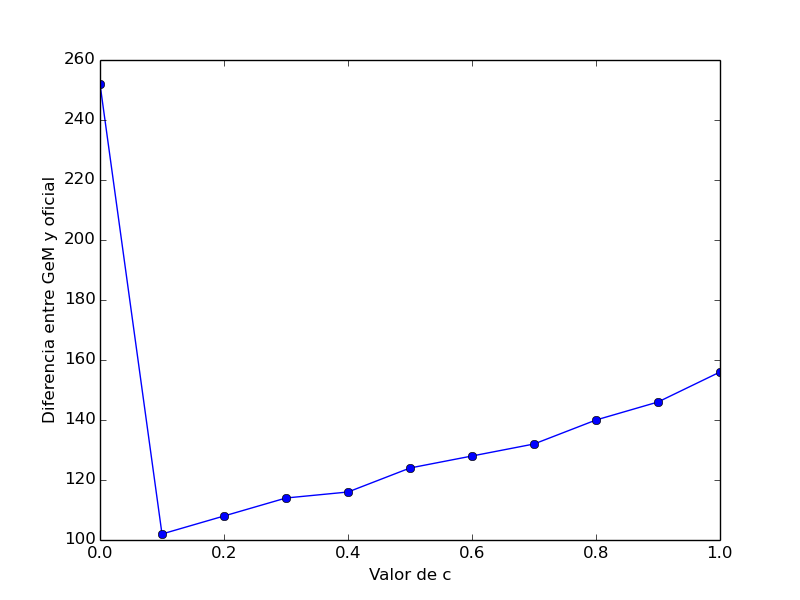
\includegraphics[width=.5\textwidth]{exp6_arg.png}}
            }
        \end{figure}

        \par La posición de San Martín de San Juan (13º según el puntaje
        oficial) en el ranking GeM se debe, en parte, a que le ganó a San
        Lorenzo en la fecha 3, mientras que Aldosivi (24º según el puntaje
        oficial) logró lo mismo en la fecha 10 y le gano a San Martín de San
        Juan en la fecha 22. Removiendo esos partidos sus posiciones en GeM
        bajan significativamente.

        \par De todos modos podemos observar que, para el valor de $\alpha=0.1$,
        el ranking devuelto por GeM se parece un poco más al oficial, d\'andonos
        los 6 primeros puestos que se pueden observar en el cuadro
        \ref{subfig:exp6_arg_prim}.

        \begin{figure}[H]
            \centering
            \caption{GeM vs Primera Divisi\'on F\'utbol Argentino para $\alpha=0.1$}
            \label{fig:exp6_arg_2}
            \subfloat[][Primeros Puestos\label{subfig:exp6_arg_prim}]{
                \footnotesize
                \setlength{\tabcolsep}{3pt}
                \begin{tabular}{|l|r||l|r|}
                    \hline
                    \multicolumn{2}{|c||}{GeM}&\multicolumn{2}{c|}{Oficial: 3-1-0}\\
                    \hline
                    Equipo & Puntaje & Equipo & Puntaje\\
                    \hline\hline
                    River Plate &0.0383429& San Lorenzo &50 \\
                    Boca Juniors& 0.038337& Boca Juniors &49 \\
                    San Lorenzo &0.0372973& Racing Club &46 \\
                    Racing Club &0.0363868& Rosario Central &45 \\
                    San Martín (SJ) &0.0352285& River Plate &44 \\
                    Rosario Central &0.0347587& Independiente &38\\
                    \hline
                \end{tabular}
            }\hspace{2pt}
            \subfloat[][\'Ultimos Puestos\label{subfig:exp6_arg_ult}]{
                \footnotesize
                \setlength{\tabcolsep}{3pt}
                \begin{tabular}{|l|r||l|r|}
                    \hline
                    \multicolumn{2}{|c||}{GeM}&\multicolumn{2}{c|}{Oficial: 3-1-0}\\
                    \hline
                    Equipo & Puntaje & Equipo & Puntaje\\
                    \hline\hline
                    Olimpo &0.0316438&Godoy Cruz &22\\
                    Huracán &0.0315532&Huracán &21\\
                    Godoy Cruz &0.0315278&Atlético de Rafaela &20\\
                    Atlético de Rafaela &0.0309498&Arsenal &17\\
                    Colón &0.0308694&Nueva Chicago &14\\
                    Nueva Chicago &0.0307189&Crucero del Norte &14\\
                    \hline
                \end{tabular}
            }
        \end{figure}
        \medskip

        \par De estos 6 primeros puestos de GeM, 5 efectivamente corresponden a
        esos primeros 6 lugares según el oficial (el que falta es Independiente,
        que GeM ubica 15º) y uno de ellos está en la misma posición en ambos
        rankings.

        \par Otra coincidencia notable son los últimos puestos, los cuales se
        pueden observar en el cuadro \ref{subfig:exp6_arg_ult}. Esta tabla tiene
        3 coincidencias débiles (mismos equipos en distinta posición) y una
        coincidencia exacta.\\

%%*************************************************************************
    \item En este caso, la diferencia para valores no nulos de $\alpha$ 
        es escasa, y la diferencia con el oficial en general es mucho mejor que
        para el caso del campeonato argentino. Consideramos esto relacionado al
        hecho de que hay pocos partidos en total, y a que la organización del
        torneo también se basa fuertemente en la transitividad de victorias (al
        menos en la fase final): en un Mundial, si A le ganó a B y B a C, se asume que A es
        mejor que C. 
        
        \par Para todos los valores no nulos de $\alpha$ GeM ubicó
        correctamente como ganador a Alemania. Para $\alpha=0.1$ considero que
        el subcampeón fue Países Bajos, lo cual sorprende dado que Argentina le
        ganó ''4 a 2'' (el resultado de los penales). Evidentemente un valor tan
        bajo de $\alpha$ le da baja importancia a esto y pondera más las
        diferencias de goles de Países Bajos contra sus rivales (4 vs España, 2
        vs Chile), mucho mejores que las de Argentina (que ganó todos sus
        otros partidos por un gol de diferencia). Para todos los demás valores de
        $\alpha$, GeM identificó correctamente a Argentina como subcampeón.

        \par Las menores diferencias generales se obtuvieron para $\alpha=0.2$,
        $\alpha=0.3$ y $\alpha=0.4$ ''empatadas'' en una distancia de 50 con el
        ranking oficial de la FIFA. En estos casos sorprende la precisión de los
        resultados. Por ejemplo, observemos los primeros 8 lugares en la
        siguiente tabla, que coinciden exactamente con el ranking provisto por
        la FIFA:

        \begin{figure}[H]
            \centering
            \caption{GeM vs Copa del Mundo 2014}
            \subfloat[][Primeros puestos $\alpha=0.4$]{
                \footnotesize
                \setlength{\tabcolsep}{3pt}
                \begin{tabular}[b]{|l|r|}
                    \hline
                    Equipo & Puntaje\\
                    \hline\hline
                    Alemania &0.0986858\\
                    Argentina &0.0764719\\
                    Países Bajos &0.0650904\\
                    Brasil &0.0480157\\
                    Colombia& 0.0419815\\
                    Bélgica &0.0405001\\
                    Francia &0.0396461\\
                    Costa Rica &0.0344357\\
                    \hline
                \end{tabular}
            }\hspace{10pt}
            \subfloat[][Diferencia en Funci\'on de $\alpha$]{
                \raisebox{-.13\height}{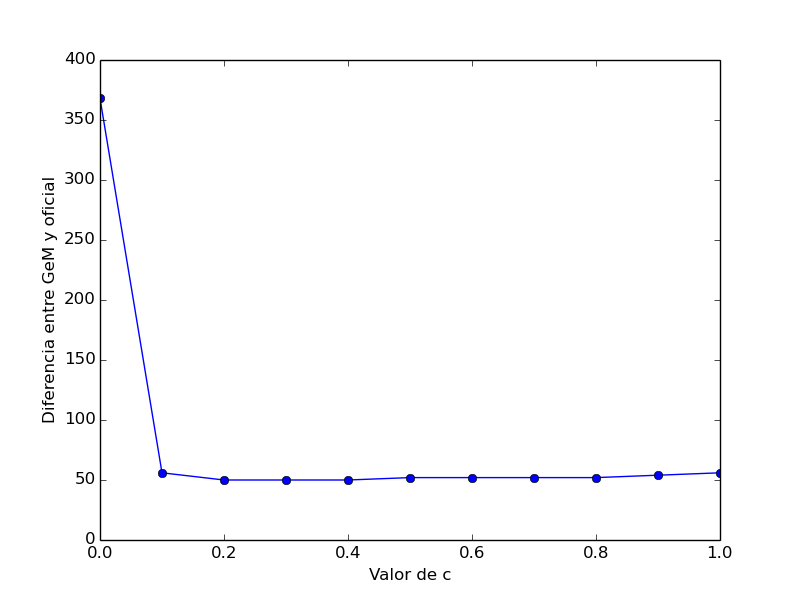
\includegraphics[width=0.5\textwidth]{exp6_2014.png}}
            }
        \end{figure}
        
        Al consultarle su opinión al respecto de si fue o
        no penal, GeM guardó un respetuoso silencio.

%%*************************************************************************
    \item Nuevamente observamos una buena aproximación entre GeM y el ranking
        oficial. Quizás los más sorprendente es que para todos los valores no
        nulos de $\alpha$, GeM supo clasificar a Alemania Federal como el
        ganador del torneo a pesar de haber perdido por una diferencia de 5
        goles en la fase de grupos con el subcampeón Hungría. La explicación que
        le encontramos a esto se basa en que la final se disputó precisamente
        entre esos dos equipos, y Alemania Federal se consagró ganador por 3 a
        2. Esto produce que el grafo de conectividad tenga un ciclo entre esas
        dos selecciones, lo cual hace que parte del "puntaje" de Hungría vuelva
        a Alemania Federal. Todo eso sumado a la excelente campaña de este
        último en el campeonato (4 a 1 vs Turquía, 7 a 2 nuevamente vs Turquía,
        2 a 0 vs Yugoslavia y 6 a 1 vs Austria, que venía de ganar varios
        partidos también por gran diferencia) lo posiciona efectivamente como
        ganador según GeM.

        \par También para todos los valores de $\alpha$ GeM acierta en ubicar a
        Hungría como subcampeón.

        \par La menor diferencia con el ranking oficial se obtiene con
        $\alpha=0.8$ y $\alpha=0.9$. Es preciso notar que no pudimos evaluar el
        caso $\alpha=1$ por no converger para esta instancia, a diferencia de
        las dos competiciones anteriores\footnote{Sabemos por la secci\'on
        \ref{sec:introduccion} que la convergencia está asegurada solo para $0\leq\alpha <1$, pero de todos modos venimos
        ``ensayando'' con $\alpha=1$ sabiendo que dicho valor no tiene por qué hacer
        converger al m\'etodo de la potencia para nuestro $M$}.

        \par En estos dos casos, GeM acertó en los 5 primeros puestos de la
        competición, siendo estos:

        \begin{figure}[H]
            \centering
            \caption{GeM vs Copa del Mundo 1954}
            \subfloat[][Primeros Puestos $\alpha=0.4$]{
                \footnotesize
                \setlength{\tabcolsep}{3pt}
                \begin{tabular}{|l|r|}
                    \hline
                    Equipo & Puntaje\\
                    \hline\hline
                    Alemania Federal &0.421402\\
                    Hungría &0.409884\\
                    Austria &0.0299615\\
                    Uruguay &0.0252637\\
                    Suiza &0.0169375\\
                    \hline
                \end{tabular}
            }\hspace{10pt}
            \subfloat[][Diferencia en Funci\'on de $\alpha$]{
                \raisebox{-.5\height}{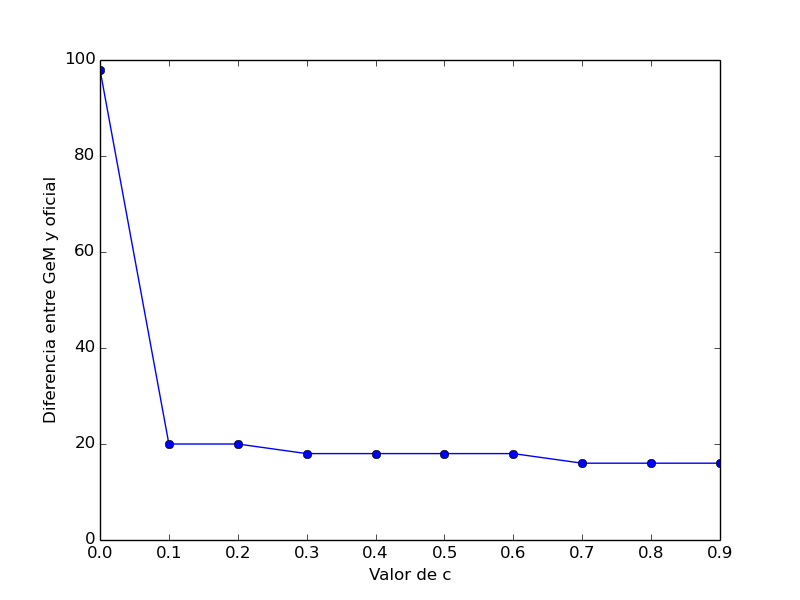
\includegraphics[width=0.5\textwidth]{exp6_1954.png}}
            }
        \end{figure}
\end{enumerate}
\medskip

%%*************************************************************************
\par Lo m\'as jugoso de toda esta experimentaci\'on radica en que comparamos el
modelo GeM de rankings contra todos rankings oficiales que est\'an vigentes. El
primer resultado interesante es observar que GeM est\'a mucho m\'as cerca para
del ranking utilizado en las copas del mundo que del torneo actual del f\'utbol
argentino, y esto se ve para cualquier $\alpha\neq 0$ (el caso con $\alpha = 0$,
como ya se comentado en experimentos previos, concibe un modelo donde todos los
equipos le pueden ganar a todos con la misma probabilidad, sin importar los
resultados previos, haciendo a este par\'ametro poco interesante para analizar
por su obvia ignorancia de la realidad\footnote{¿O acaso las chances de que
Racing le gane a Crucero del Norte son las mismas de que pierda?}). A\'un as\'i,
a pesar de esta distancia, vemos que en el caso del torneo de f\'utbol
argentino, su ranking en los extremos de la ''tabla'' (particularmente en el
extremo inferior) suele ubicar a los mismos equipos que el ranking oficial. Esto
nos indica que a pesar de tener rankings muy distintos, en t\'erminos generales
ambos rankings diferencian de forma similar a los equipos ''buenos'' y
''malos''.

\par Concluyendo, vemos que GeM puede o no parecerse a otros rankings oficiales,
pero la determinaci\'on de si es mejor o peor depender\'a de qué opinen quienes
lo utilicen. Lo que si podemos afirmar es que GeM tiende a aproximarse m\'as
a los rankings oficiales (al menos los vistos) en los extremos del mismo. Es
decir, a pesar de estar a una distancia no despreciable del ranking oficial, los
equipos se\~nalados como los m\'as fuertes o mejores por ambos rankings (o los
peores) tienen varias coincidencias. Decimos entonces que, desde el punto de
vista de clasificar a un equipo como ''de los buenos'' o ''de los malos'' de la
competencia, cualquiera de los rankings dar\'ia resultados similares, pero estos
se diferencian al entrar en el detalle de qué equipo es mejor que otro.
